\documentclass{article}
\usepackage[utf8]{inputenc}
\usepackage{amsmath}
\usepackage{graphicx}
\usepackage[colorlinks=true]{hyperref}
\usepackage{cleveref}
\graphicspath{ {./images/} }
\setlength{\parindent}{0pt}

\title{Dynamics of ``problem-place'' disease spread}
\author{}
\date{}

\begin{document}

\maketitle

\begin{abstract}
Disease transmission is not homogeneous: in any outbreak a small
number of infected individuals
are responsible for a disproportionately large number of subsequent
infections.
This is certainly the case in COVID-19, in which 20\% of infections may cause
as many as 85\% of secondary infections[citation?].
However, our mechanistic understanding
of this phenomenon – known as super-spreading – is limited[citations?].

Here we introduce and analyze
a simple model of an outbreak with super-spreading via "problem-place" locations:
disease spreads homogeneously throughout the population at a low rate, but
spreads rampantly at certain locations (bars, restaurants, churches, etc.)
that individuals visit daily with their own fixed probabilities.

Compared to homogeneous dynamics, outbreaks are less
likely to happen but are accelerated when they do occur; causing larger
outbreaks in some cases, but paradoxically smaller and less sever outbreaks 
in moderately to highly infectious diseases.
\end{abstract}


\section{Introduction}

Disease superspreading is well documented and even in some cases quantified.
However, our primary mechanistic understanding of it hinges on some individuals
simply being much more infectious – either by having many more connections or
simply by literally spreading a higher viral load. The latter scenario is 
not born out by the data [see paper on size of lungs, etc].
The former scenario leaves some interesting mechanics unexplored.

In any case, 

\section{Methods}
\subsection{Models}

\begin{itemize}
\item SIR is used throughout
\item ABM pseudocode
\item differential equation system
\item difference equation system
\end{itemize}

\subsection{Riskiness Distributions}

See \Cref{fig:risk_distributions}.


\begin{figure}
\centering
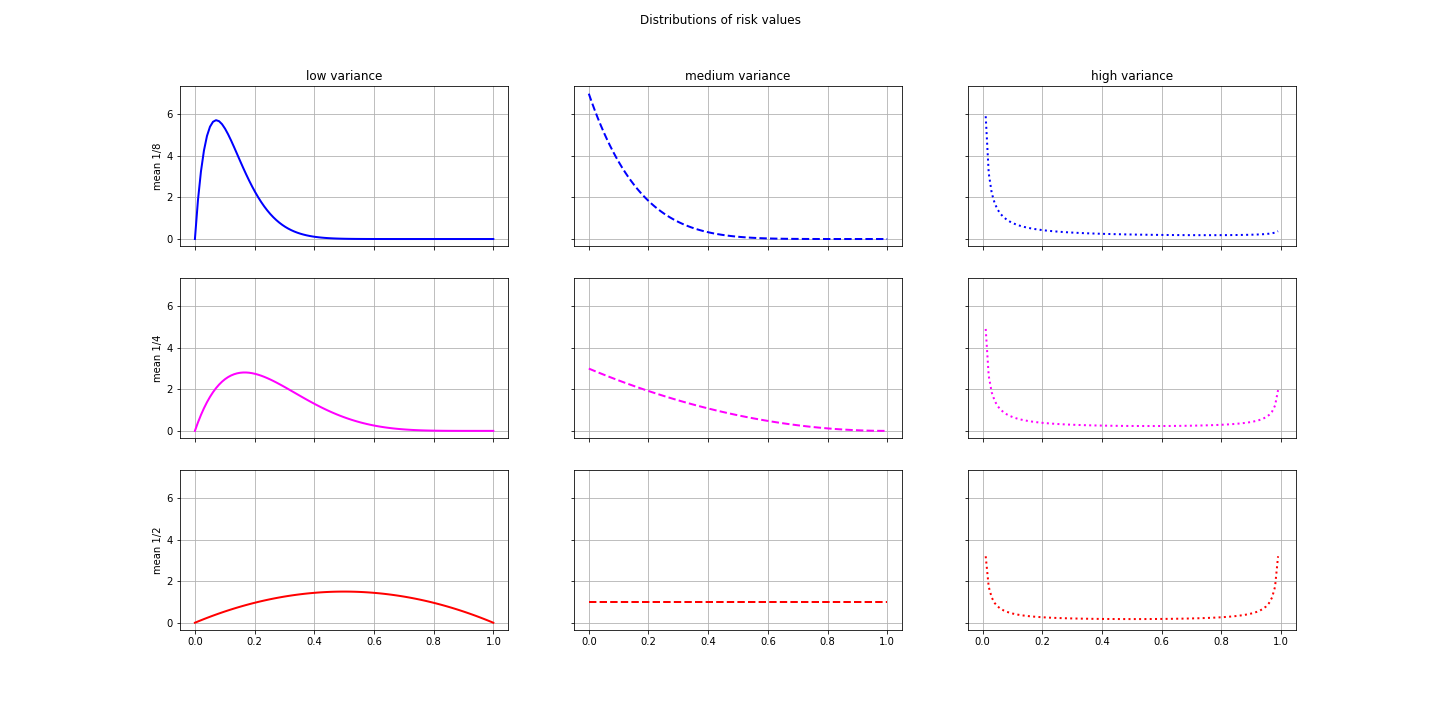
\includegraphics[width=\textwidth]{risk_distributions}
\caption{This is the risk distributions figure}
\label{fig:risk_distributions}
\end{figure}

\subsection{$\mathcal{R}_0 = \mathcal{C}_0 + \mathcal{P}_0$}


\section{Results}
\subsection{Extinction Probability}


% Define: What is disease extinction?
How does extinction probability change in the problem place model?\\

We consider three scenarios: problem place spread is responsible (initally)
for 25\%, 50\% or 75\% of total disease spread. For each, we vary $\mathcal{R}_0$
from 0 to 8, and run a simulation 1000 times. One individual chosen
at random becomes infected and we run the simulation until all infeceted
individuals have recovered and record this total number of infected individuals.\\

These numbers are genarally bimodal – with simulations
ending at either 20 or fewer total recovered, or greater than 500 total
recovered – so we can categorize each simulation as containing an extinction
or an outbreak (using a threshold of 50 total recovered).\\

These results are all shown in \Cref{fig:extinction_results} for each of the riskiness
distributions discussed in the introduction.\\


\begin{figure}
\centering
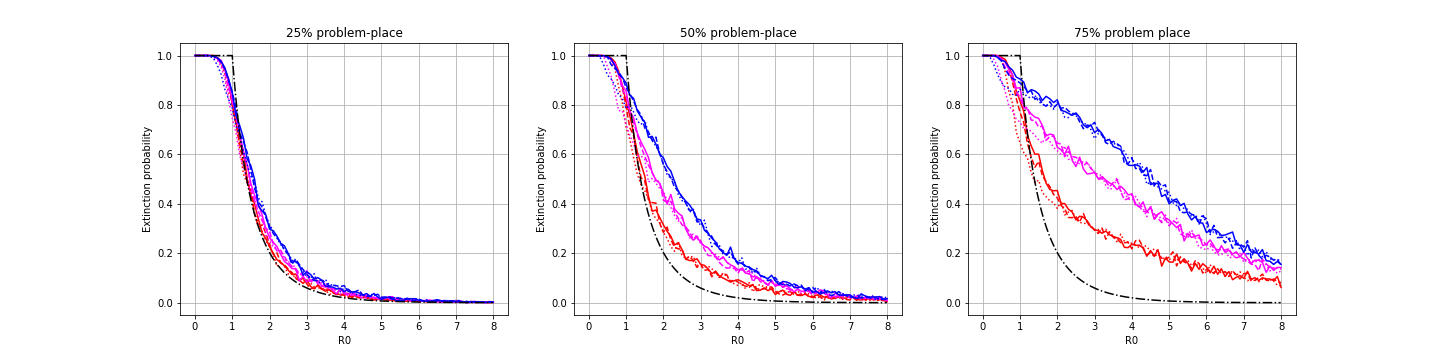
\includegraphics[width=\textwidth]{extinction_results}
\caption{Extinction Results}
\label{fig:extinction_results}
\end{figure}



We find that higher problem place spread means an outbreak is overall less
likely (extinction probability is greater). We find that this effect is
more pronounced the lower the mean risk taking in the population. And we see,
surprisingly, that the effect is exactly the same \textit{between} scenarios
with the same mean riskiness even if their distributions otherwise vary
significantly (lines of the same color overlap).


To explain these results, we approximate the simulation with a branching process
(derivation is shown in the appendix)
and find that we can compute the "extinction" probability of a given simulation
$\tau$ as:

\begin{equation}
\tau = ... \tau
\label{eqn:extinction}
\end{equation}


\begin{figure}
\centering
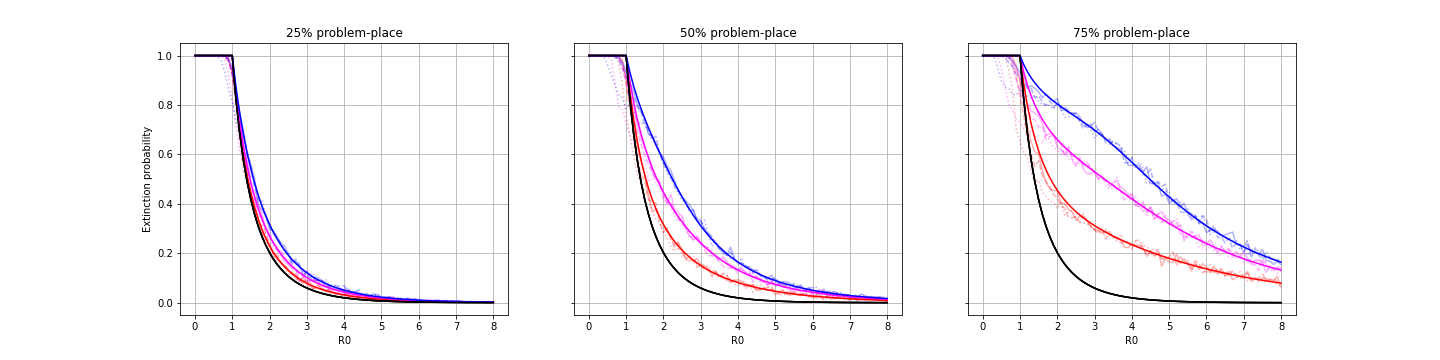
\includegraphics[width=\textwidth]{extinction_explained}
\caption{Extinction Explained. Predictions according to \Cref{eqn:extinction}
drawn in solid color over simulation results from \Cref{fig:extinction_results}.}
\label{fig:extinction_explained}
\end{figure}




These predictions are shown in \Cref{fig:extinction_explained} compared
to the simulated results from \Cref{fig:extinction_results}, showing
great agreement. So what does this tell us?\\


The branching process approximation depends only on the mean risk
$\bar\rho_s$ in the population and not on any other aspects of
the distribution. This tells us the variance and shape of the distribution
are more of secondary effects. They may be important in other contexts (and
we'll see later that they are), but they don't impact the likilihood of an
outbreak – the only things that matter are the infectiousness parameters
$\beta_c$ and $\beta_r$, and the expected number of people in the problem place,
not whether those same people will be back the next day, etc. By the time
these more secondary effects come into play there's already a second
wave of infections and disease extinction has become extremely unlikely.



\subsection{Outbreak Metrics}

Next we look at only those scenarios in which an outbreak occurs and ask how
problem place dynamics affect the size and severity of the outbreak. We consider
Max I – the peak number of infected individuals – and Final R – the total number
individuals infected (and recovered) over the entire course of the outbreak.
Similar to [Extinction Probability Section] we fix a value of $\mathcal{R}_0$, then for
the risk distributions discussed in [Intro Section] we vary the contribution
of problem place spread and observe the effects. This is shown in \Cref{fig:outbreak_results},
and the results thereof are summarized in [Table 1].



\begin{figure}
\centering
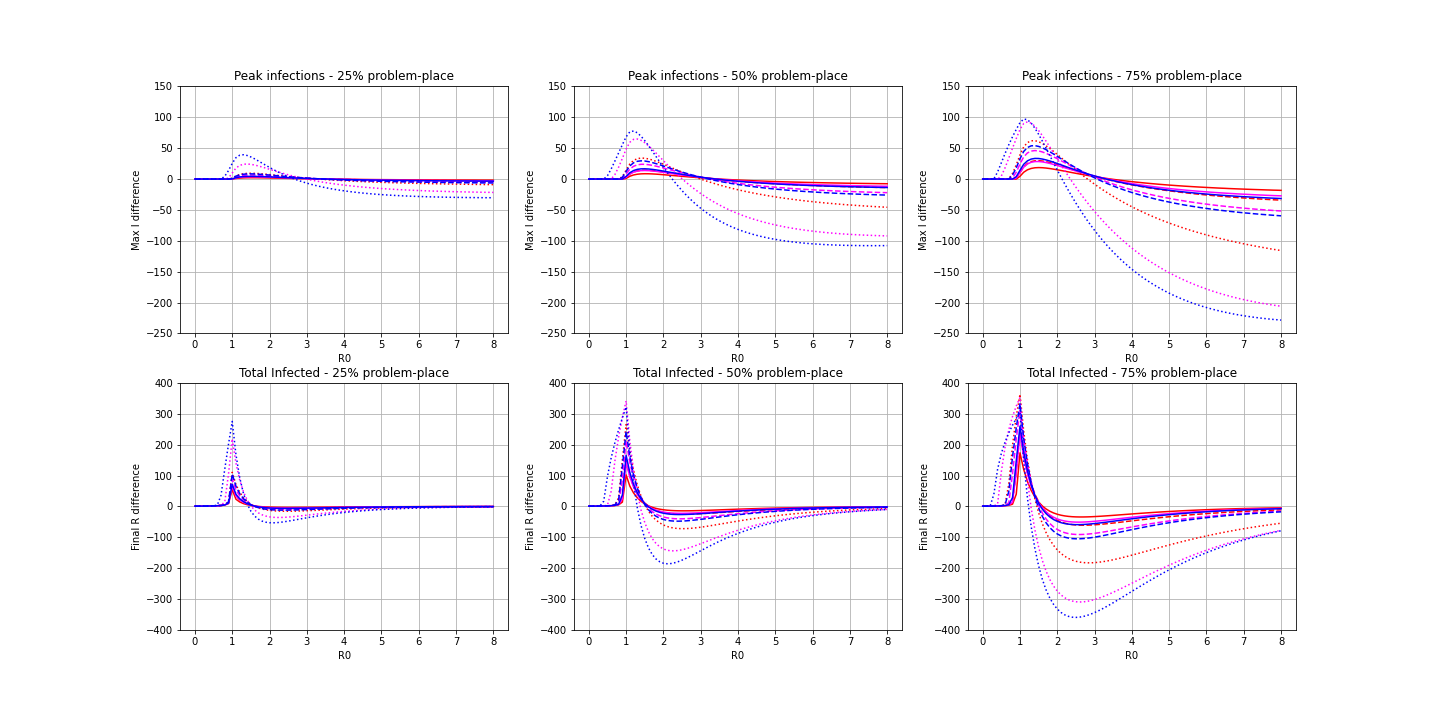
\includegraphics[width=\textwidth]{outbreakresults}
\caption{Outbreak Results}
\label{fig:outbreak_results}
\end{figure}

% \pagebreak
% outcome                  low R0       medium R0    high R0
% ---------------------   -------      ---------    --------
% outbreak probability    decreased     decreased    decreased
% peak infections         _increased_    _increased_    decreased
% total infections        _increased_    decreased    decreased

\subsection{Disease Evolution}

How can we explain these findings?

Here the differential equation model is useful.

In a more traditional compartment model, we can find $R(t)$ – the instantaneous
expected number of secondary infections caused by a new infection at time t.

In the analysis section we show that the basic reproduction number $R(t)$ is
given by:

$$R(t) = \frac{\bar S}{\gamma} \left( \beta_c
		+ \beta_r \bar \rho_S \bar \rho_I \right)$$

where $\bar\rho_S$ and $\bar\rho_I$ are the means of riskiness in the $S$ and
$I$ populations. We also show that


\begin{equation}
\frac{d\bar\rho_S}{dt} = 
\end{equation}

and

$$\frac{d\bar\rho_I}{dt} = ...$$

so that $\bar\rho_S$ always decreases at a rate proportional to the
variance of $\rho_S$ at the time, and that $\bar\rho_I$ is forced towards
some value between $\bar\rho_S$ and $\bar\rho_S + \frac{Var(\rho_S)}{\bar\rho_S}$
– which may be much larger than $\bar\rho_S$, but must necessarily increase
initially and later decrease.


The results of this difference are shown for three different values of $R_0$,
alongside $R_t$
and $\beta_{effective}(\bar\rho_I, \bar\rho_S)$ in [Figure 1].

From here we can see what's causing [results from the previous section – Figure 2].

These results are shown for three $R_0$ scenarios in [Figure 2].

\section{Analysis} 



\subsection{Disease Extinction}

Given a disease with $R0$ of 2, the standard SIR model predicts an
outbreak to infect 79.681\% of the population before running its course.
When we simulate such an outbreak (homogeneous, with $R0$ of 2) in a population
of 1,000, we see outbreaks of about this size (shown in Figure 1.), 
but we also see some number of simulations in which there's no large outbreak at all.

%![Figure 1. figure showing histogram of outbreak sizes](images/extinction_histogram.png)

We can predict the probability of a large vs small outbreak with reasonable
accuracy by replacing the outbreak scenario with a similarly parameterized
branching process. These predictions are shown against the simulated results
in Figure 2.

% [^1]: In the homogeneous simulation, an infected individual has 
% probability $p(n)$ of infecting $n$ individuals before recovering, where
% $p(n)$ is nearly the probability mass function of the binomial distribution
% with parameters $\beta$ (infectiousness) and $N$ (total population);
% except that $N$ is not correct since not every individual is susceptible and
% things are further complicated by the possibility of multiple infected
% invididuals at once. In the branching process, $p(n)$ is exactly the
% probability mass function of the binomial distribution with parameters $\beta$
% and $N$. So to find the probability of extinction $\gamma$, we follow the normal
% formula:

% 	$$
% 	\begin{aligned}
% 	\gamma &= p(0) + p(1) \gamma + p(2) \gamma^2 + ... + p(N) \gamma^N\\
% 	\gamma &= G_{Binomial(\beta, N)}(\gamma)\\
% 	\gamma &= (1 - \beta + \beta \gamma)^N\\
% 	\end{aligned}
% 	$$
% 	This can be easily computed and is how we produce the approximation in Figure 2.


Let X be a random variable that represents the number of infections caused by
a single infected individual with riskyness $\rho_i$ before recovering, and
let $j = 1, \ldots, N$ index the susceptible population so that $\rho_j$ is the
riskyness of individual $j$.

Then 
$$P(X = 0) = (1 - \rho_i) [ (1 - \beta_c)^N ] + \rho_i [ \prod_j (1 - (\beta_c + \beta_r \rho_j)) ]$$

By assumption riskyness for each individual is drawn independently from one
distribution, so in expectation (over riskyness values) this is:


\begin{align*}
E[P(X = 0)] &= E[(1 - \rho_i) [ (1 - \beta_c)^N ] + \rho_i [ \prod_j (1 - (\beta_c + \beta_r \rho_j)) ]]\\
&= (1 - E[\rho_i]) [ (1 - \beta_c)^N ] + E[\rho_i] [ \prod_j (1 - (\beta_c + \beta_r E[\rho_j])) ]]\\
&= (1 - \bar\rho) [ (1 - \beta_c)^N ] + \bar\rho [(1 - (\beta_c + \beta_r \bar\rho))^N ]\\
&= (1 - \bar\rho) B(\beta_c, N, 0) + \bar\rho B(\beta_c + \bar\rho \beta_r, N, 0)\\
\end{align*}

Where $B(a, b, x)$ is the Binomial probability mass at x with parameters a and b.

Similarly, $E[P(X) = x]$ is given by

$$(1 - \bar\rho) B(\beta_c, N, x) + \bar\rho B(\beta_c + \bar\rho \beta_r, N, x)$$


So


\begin{align*}
G_X(s) &= P(X=0) + P(X=1)s + P(X=2)s^2 + \ldots\\
&= [\bar\rho B_1(0) + (1 - \bar\rho)B_2(0)] + [\bar\rho B_1(1) + (1 - \bar\rho)B_2(1)]s + [\bar\rho B_1(2) + (1 - \bar\rho)B_2(2)]s^2 + \ldots\\
&= \bar\rho G_{B_1}(s) + (1 - \bar\rho)G_{B_2}(s)\\
&= \bar\rho [(1 - \bar\rho \beta_r)(1 - \beta_c) + 
				(1 - (1 - \bar\rho \beta_r)(1 - \beta_c) s]^N + 
   (1 - \bar\rho)[(1 - \beta_c) + \beta_c s]^N\\
\tau &= \bar\rho [(1 - \bar\rho \beta_r)(1 - \beta_c) + 
				(1 - (1 - \bar\rho \beta_r)(1 - \beta_c) \tau]^N + 
   (1 - \bar\rho)[(1 - \beta_c) + \beta_c \tau]^N\\
\end{align*}


% For small $\beta_c + \bar\rho \beta_r$, the overlap is very small so:

% $$ 
% \begin{aligned}
% P(X = x) &\approx (1 - \bar\rho) B(\beta_c, N, x) + \bar\rho (B(\beta_c, N, x) + B(\bar\rho \beta_r, N, x))\\
% &= \bar\rho B(\bar\rho \beta_r, N, x) + B(\beta_c, N, x)\\
% \end{aligned}
% $$

% And

% $$
% \begin{aligned}
% G_X(s) &\approx \bar\rho [(1 - \bar\rho \beta_r) + 
% 				\bar\rho \beta_r s]^N + [(1 - \beta_c) + \beta_c s]^N\\
% \tau &\approx \bar\rho [(1 - \bar\rho \beta_r) + 
% 				\bar\rho \beta_r \tau]^N + [(1 - \beta_c) + \beta_c \tau]^N
% \end{aligned}
% $$

\subsection{Outbreak Dynamics}

\subsubsection{Some initial definitions/conveniences}

Initial equations:


\begin{align*}
\frac{\partial S(\rho, t)}{\partial t} &=
	-\beta_c S(\rho, t) \int_{0}^1 I(u, t) du
	-\beta_r S(\rho, t) \rho \int_{0}^1 I(u, t) u du\\
\frac{\partial I(\rho, t)}{\partial t} &=
	\beta_c S(\rho, t) \int_{0}^1 I(u, t) du
	+ \beta_r S(\rho, t) \rho \int_{0}^1 I(u, t) u du - \gamma I(p, t)
\end{align*}


For convenience, we introduce the following shorthands 
for the "moments" of $I(\rho)$ and $S(\rho)$:


\begin{align*}
\bar S &:= \int_{0}^{1} S(\rho) d\rho
	& \bar I &:= \int_{0}^{1} I(\rho) d\rho\\
\hat S &:= \int_{0}^{1} S(\rho) \rho d\rho
	& \hat I &:= \int_{0}^{1} I(\rho) \rho d\rho\\
\hat{\hat{ S}} &:= \int_{0}^{1} S(\rho) \rho^2 d\rho
	& \hat{\hat{ I}} &:= \int_{0}^{1} I(\rho) \rho^2 d\rho\\
\vdots & & \vdots \\
\overset{(n)}{S} &:= \int_{0}^{1} S(\rho) \rho^n d\rho
	& \overset{(n)}{I} &:= \int_{0}^{1} I(\rho) \rho^n d\rho\\
\end{align*}


Now we can more concicely write the initial equations:


\begin{align*}
\frac{\partial S(\rho, t)}{\partial t} &=
	-\beta_c S(\rho, t) \bar I
	-\beta_r S(\rho, t) \rho \hat I\\
\frac{\partial I(\rho, t)}{\partial t} &=
	\beta_c S(\rho, t) \bar I
	+ \beta_r S(\rho, t) \rho \hat I - \gamma I(p, t)
\end{align*}


Finally, notice that $S(\rho)$ and $I(\rho)$ are defined over $\rho \in [0, 1]$,
and that these give the population at a given risk level. We can equivalently
think of how risk is distributed over the S and I populations:\\

We introduce $\rho_S$ and $\rho_I$: these are random variables drawn from
the distributions of risk in the S and I populations, respectively.

The means of these variables are:

\begin{align*}
\bar\rho_S
&= \frac{\int_{0}^{1} S(\rho) \rho d\rho}{\int_{0}^{1} S(\rho) d\rho}
= \frac{\hat S}{\bar S}\\
\bar\rho_I
&= \frac{\int_{0}^{1} I(\rho) \rho d\rho}{\int_{0}^{1} I(\rho) d\rho}
= \frac{\hat I}{\bar I}\\
\end{align*}

(This is just setting up interpretable variables for the terms
$\frac{\hat S}{\bar S}$ and $\frac{\hat I}{\bar I}$, which start to pop up
in a bunch of places.)\\


\subsubsection{Moments equations}

First we have a general result relating the "moments" of S and I.

% TODO - arrive at this by integration (maybe start with the 0)

Suppose we want to know how the total susceptible population is changing. We
can integrate $\frac{\partial S}{\partial t}$ over $\rho$:

\begin{align*}
\frac{d \bar{S}}{dt} = \int_{0}^{1} \frac{\partial S(\rho)}{\partial t} d\rho
&= \int_{0}^{1} (-\beta_c S(\rho) \bar I - \beta_r S(\rho) \rho \hat I) d\rho  \\
&= -\beta_c (\int_{0}^{1} S(\rho) d\rho) \bar I
	- \beta_r (\int_{0}^{1} S(\rho) \rho d\rho) \hat I\\
&= -\beta_c \bar S \bar I - \beta_r \hat S \hat I
\end{align*}

Similary, we can find that:

$$\frac{d \bar{I}}{dt} = \int_{0}^{1} \frac{\partial I(\rho)}{\partial t} d\rho
= \beta_c \bar S \bar I + \beta_r \hat S \hat I - \gamma \bar I$$\\

If we want to see how the first moments are changing, we follow a similar method:

\begin{align*}
\frac{d \hat{S}}{dt} = \int_{0}^{1} \frac{\partial S(\rho)}{\partial t} \rho d\rho
&= \int_{0}^{1} (-\beta_c S(\rho) \bar I - \beta_r S(\rho) \rho \hat I) \rho d\rho  \\
&= -\beta_c (\int_{0}^{1} S(\rho) \rho d\rho) \bar I
	- \beta_r (\int_{0}^{1} S(\rho) \rho^2 d\rho) \hat I\\
&= -\beta_c \hat S \bar I - \beta_r \hat{\hat{ S}} \hat I
\end{align*}\\

And for any general moment:


\begin{equation}
\label{eqn:moments}
\begin{aligned}
\frac{d \overset{(n)}{S} }{dt} &=
	-\beta_c \overset{(n)}{S} \bar I
	-\beta_r \overset{(n+1)}{S} \rho \hat I \\
\frac{d \overset{(n)}{I}}{dt} &=
	\beta_c \overset{(n)}{S} \bar I
	+ \beta_r \overset{(n+1)}{S} \rho \hat I - \gamma \overset{(n)}{I}
\end{aligned}
\end{equation}


\subsubsection{Basic Reproduction Number}

In the homogeneous SIR model, the basic reproduction number (number of secondary
infections per infection) is:

$$\mathcal{R}_t = \frac{S\beta}{\gamma}$$

In this model, we can derive a similar form for the expected
number of secondary infections per infection by dividing $\frac{d \bar S}{dt}$
by $\hat I$ (current number of infected individuals) then multiplying by
the mean duration of an infection $\frac{1}{\gamma}$.

\begin{align*}
\mathcal{R}_t &= -\frac{d\bar S}{dt} \frac{1}{\gamma \bar I} \\
	&= \frac{1}{\gamma} \beta_c \bar S \frac{\bar I}{\bar I}
		+ \frac{1}{\gamma} \beta_r \hat S \frac{\hat I}{\bar I}\\
	&= \frac{1}{\gamma} \bar S\left( \beta_c
		+ \beta_r \frac{\hat S}{\bar S} \frac{\hat I}{\bar I} \right)\\
	&= \frac{1}{\gamma} \bar S\left( \beta_c
		+ \beta_r \bar \rho_S \bar \rho_I \right)\\
\end{align*}

This gives a nicely analogous result, where the homogenous $\beta$ is
replaced by what we can think of as an effective $\beta$:
$(\beta_c + \beta_r \bar \rho_I \bar\rho_S)$, which is a straightforward
function of both $\beta$ terms and the mean riskiness in both populations.\\

We then would like to know how $\bar\rho_S$ and $\bar\rho_I$ are changing.
We'd expect $\bar\rho_S$ (mean riskiness of the susceptible population) to
monotonically decrease, as more risk-taking- susceptible individuals are
more likely to be infected. We'd expect $\bar\rho_I$ to behave almost
like a chemostat as higher-risk- individuals flow in, and all individuals flow
out at a rate of $\gamma$. It should increase initially, and eventually decrease
after the mean of riskiness decreases sufficiently in the susceptible population.

\subsubsection{$\bar\rho_S$}

Fortunately, we can find explicit expressions for $\frac{d}{dt}\bar\rho_S$
and $\frac{d}{dt}\bar\rho_I$.\\

Start with $\frac{d\bar\rho_S}{dt}$, and differentiate:


\begin{align*}
\frac{d}{dt}\bar\rho_S
&= \frac{d}{dt} \left( \frac{\hat S}{\bar S} \right)\\
&= \frac{\frac{d}{dt} \hat S \bar S - \hat S \frac{d}{dt}\bar S}{\bar S^2}\\
&= \frac{1}{\bar S}\left(
-\beta_c\hat S \bar I - \beta_r \hat{\hat{S}}\hat I
\right)
- \frac{\hat S}{\bar S^2}\left(
-\beta_c \bar S \bar I - \beta_r \hat S \hat I
\right)\\
&= -\beta_c \frac{\hat S}{\bar S} \bar I
- \beta_r \frac{\hat{\hat{S}}}{\bar S}\hat{I}
+ \beta_c \frac{\hat S}{\bar S}\bar I
+ \beta_r \left(\frac{\hat S}{\bar S}\right)^2 \\
&= 
- \beta_r \frac{\hat{\hat{S}}}{\bar S}\hat{I}
+ \beta_r \left(\frac{\hat S}{\bar S}\right)^2 \\
&= -\beta_r \hat I \left(\frac{\hat{ \hat{ S}}}{\bar S} - \left(\frac{\hat S}{\bar S}\right)^2  \right)\\
\end{align*}

Here, notice $\hat{ \hat{ S}}$ sums $\rho^2$ over $[0, 1]$ and so
$\frac{\hat{ \hat{ S}}}{\bar S}$ we can write as $E[\rho_S^2]$. And similarly
$\frac{\hat S}{\bar S}$ = $E[\rho_S]$ so
$$
\frac{\hat{ \hat{ S}}}{\bar S} - \left(\frac{\hat S}{\bar S}\right)^2
= E[\rho_S^2] - E[\rho_S]^2 
$$

which is the variance of the riskiness of the susceptible population
$Var(\rho_S)$. This allows us to rewrite the equation as:

$$
\frac{d}{dt}\bar\rho_S = -\beta_r \hat I \text{Var}(\rho_s)
$$

or

$$
\frac{d}{dt}\bar\rho_S = -\beta_r \bar I \bar\rho_I \text{Var}(\rho_s)
$$

This confirms that $\rho_S$ decreases monotonically (as long as there is some
infected population with nonzero mean riskiness), and further shows that
it decreases proportionally to the variance of the distribution of riskiness
in the S population.

\subsubsection{$\bar\rho_I$}


% TODO - add all the stuff after applying product rule

\begin{align*}
\frac{d}{dt}\bar\rho_I
&= \frac{d}{dt} \left( \frac{\hat I}{\bar I} \right)\\
&= \frac{\frac{d}{dt} (\hat I) \bar I - \hat I \frac{d}{dt}(\bar I)}{\bar I^2}\\
&=  ...
\\
&= \bar S \left[
	\beta_c (\bar\rho_S - \bar\rho_I)
	+ \beta_r \bar\rho_S \bar\rho_I((\bar\rho_S + \frac{\text{Var}(\rho_S)}{\bar\rho_S})
		- \bar\rho_I))
\right]
\end{align*}
\end{document}
